% ------------------------------------------------------------------------------------------------------------------
% Basic configuration and packages
% ------------------------------------------------------------------------------------------------------------------
% Package for discovering wrong and outdated usage of LaTeX.
% More information to be found in l2tabu English version.
\RequirePackage[l2tabu, orthodox]{nag}
% Class of LaTeX document: {size of paper, size of font}[document class]
\documentclass[a4paper,11pt]{article}



% ------------------------------------------------------
% Packages not tied to particular normal language
% ------------------------------------------------------
% This package should improved spaces in the text
\usepackage{microtype}
% Add few important symbols, like text Celcius degree
\usepackage{textcomp}



% ------------------------------------------------------
% Polonization of LaTeX document
% ------------------------------------------------------
% Basic polonization of the text
\usepackage[MeX]{polski}
% Switching on UTF-8 encoding
\usepackage[utf8]{inputenc}
% Adding font Latin Modern
\usepackage{lmodern}
% Package is need for fonts Latin Modern
\usepackage[T1]{fontenc}



% ------------------------------------------------------
% Setting margins
% ------------------------------------------------------
\usepackage[a4paper, total={14cm, 25cm}]{geometry}





% ------------------------------------------------------
% Wonderful package PGF/TikZ
% ------------------------------------------------------
\usepackage{tikz}

% Loading arrows styles
\usetikzlibrary{arrows.meta}

% Loading library for positiong nodes
\usetikzlibrary{positioning}





% ------------------------------------------------------
% Package "hyperref"
% They advised to put it on the end of preambule
% ------------------------------------------------------
% It allows you to use hyperlinks in the text
\usepackage{hyperref}










% ------------------------------------------------------------------------------------------------------------------
% Title and author of the text
\title{Ti\textit{k}Z \& PGF Manual,
  \href{https://ctan.gust.org.pl/tex-archive/graphics/pgf/base/doc/pgfmanual.pdf}{3.1.10} \\
  {\Large Nauka i~testy. Seria~01, część~01}}

\author{Kamil Ziemian}


% \date{}
% ------------------------------------------------------------------------------------------------------------------










% ####################################################################
% Beginning of the document
\begin{document}
% ####################################################################





% ######################################
% Title of the text
\maketitle
% ######################################





% ##################
\begin{figure}

  \centering


  \begin{tikzpicture}

    \draw (0,0) -- (1,1);

  \end{tikzpicture}

  \caption{3~Tutorial: A~Petri-Net for Hagen,~01.}

\end{figure}
% ##################





% ##################
\begin{figure}

  \centering


  \begin{tikzpicture}

    \path ( 0,2) node[shape=circle,draw] {}
    ( 0,1) node[shape=circle,draw] {}
    ( 0,0) node[shape=circle,draw] {}
    ( 1,1) node[shape=rectangle,draw] {}
    (-1,1) node[shape=rectangle,draw] {};

  \end{tikzpicture}

  \caption{3~Tutorial: A~Petri-Net for Hagen,~02.}


\end{figure}
% ##################





% ##################
\begin{figure}

  \centering


  \begin{tikzpicture}

    \path node at ( 0,2) [shape=circle,draw] {}
    node at ( 0,1) [shape=circle,draw] {}
    node at ( 0,0) [shape=circle,draw] {}
    node at ( 1,1) [shape=rectangle,draw] {}
    node at (-1,1) [shape=rectangle,draw] {};

  \end{tikzpicture}

  \caption{3~Tutorial: A~Petri-Net for Hagen,~03.}


\end{figure}
% ##################





% ##################
\begin{figure}

  \centering


  \begin{tikzpicture}

    \node at ( 0,2) [circle,draw] {};

    \node at ( 0,1) [circle,draw] {};

    \node at ( 0,0) [circle,draw] {};

    \node at ( 1,1) [rectangle,draw] {};

    \node at (-1,1) [rectangle,draw] {};

  \end{tikzpicture}

  \caption{3~Tutorial: A~Petri-Net for Hagen,~04.}


\end{figure}
% ##################





% ##################
\begin{figure}

  \centering


  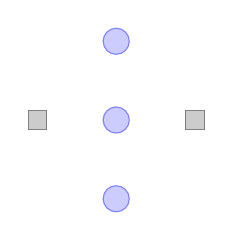
\begin{tikzpicture}

    \node at ( 0,2) [circle,draw=blue!50,fill=blue!20] {};

    \node at ( 0,1) [circle,draw=blue!50,fill=blue!20] {};

    \node at ( 0,0) [circle,draw=blue!50,fill=blue!20] {};

    \node at ( 1,1) [rectangle,draw=black!50,fill=black!20] {};

    \node at (-1,1) [rectangle,draw=black!50,fill=black!20] {};

  \end{tikzpicture}

  \caption{3~Tutorial: A~Petri-Net for Hagen,~05.}


\end{figure}
% ##################





% ##################
\begin{figure}

  \centering


  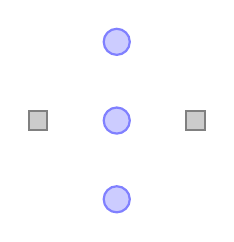
\begin{tikzpicture}
    [place/.style={circle,draw=blue!50,fill=blue!20,thick},
    transition/.style={rectangle,draw=black!50,fill=black!20,thick}]


    \node at ( 0,2) [place] {};

    \node at ( 0,1) [place] {};

    \node at ( 0,0) [place] {};

    \node at ( 1,1) [transition] {};

    \node at (-1,1) [transition] {};

  \end{tikzpicture}

  \caption{3~Tutorial: A~Petri-Net for Hagen,~06.}


\end{figure}
% ##################





% ##################
\begin{figure}

  \centering


  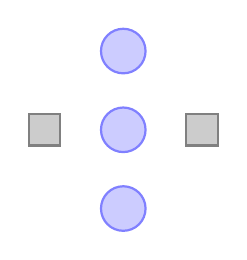
\begin{tikzpicture}
    [inner sep=2mm,
    place/.style={circle,draw=blue!50,fill=blue!20,thick},
    transition/.style={rectangle,draw=black!50,fill=black!20,thick}]


    \node at ( 0,2) [place] {};

    \node at ( 0,1) [place] {};

    \node at ( 0,0) [place] {};

    \node at ( 1,1) [transition] {};

    \node at (-1,1) [transition] {};

  \end{tikzpicture}

  \caption{3~Tutorial: A~Petri-Net for Hagen,~07.}


\end{figure}
% ##################





% ##################
\begin{figure}

  \centering


  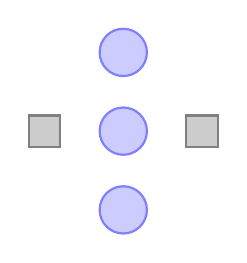
\begin{tikzpicture}
    [place/.style={circle,draw=blue!50,fill=blue!20,thick,
      inner sep=0pt,minimum size=6mm},
    transition/.style={rectangle,draw=black!50,fill=black!20,thick,
      inner sep=0pt,minimum size=4mm}]



    \node at ( 0,2) [place] {};

    \node at ( 0,1) [place] {};

    \node at ( 0,0) [place] {};

    \node at ( 1,1) [transition] {};

    \node at (-1,1) [transition] {};

  \end{tikzpicture}

  \caption{3~Tutorial: A~Petri-Net for Hagen,~08.}


\end{figure}
% ##################





% ##################
\begin{figure}

  \centering


  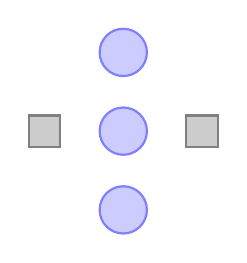
\begin{tikzpicture}
    [place/.style={circle,draw=blue!50,fill=blue!20,thick,
      inner sep=0pt,minimum size=6mm},
    transition/.style={rectangle,draw=black!50,fill=black!20,thick,
      inner sep=0pt,minimum size=4mm}]



    \node (waiting 1)      at ( 0,2) [place] {};

    \node (critical 1)     at ( 0,1) [place] {};

    \node (sempahore)      at ( 0,0) [place] {};

    \node (leave critical) at ( 1,1) [transition] {};

    \node (enter critical) at (-1,1) [transition] {};

  \end{tikzpicture}

  \caption{3~Tutorial: A~Petri-Net for Hagen,~09.}


\end{figure}
% ##################





% ##################
\begin{figure}

  \centering


  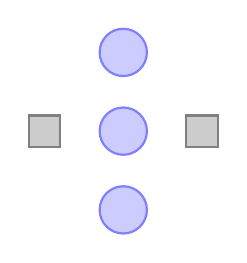
\begin{tikzpicture}
    [place/.style={circle,draw=blue!50,fill=blue!20,thick,
      inner sep=0pt,minimum size=6mm},
    transition/.style={rectangle,draw=black!50,fill=black!20,thick,
      inner sep=0pt,minimum size=4mm}]



    \node[place]      (waiting 1)      at ( 0,2) {};

    \node[place]      (critical 1)     at ( 0,1) {};

    \node[place]      (semaphore)      at ( 0,0) {};

    \node[transition] (leave critical) at ( 1,1) {};

    \node[transition] (enter critical) at (-1,1) {};

  \end{tikzpicture}

  \caption{3~Tutorial: A~Petri-Net for Hagen,~10.}


\end{figure}
% ##################





% ##################
\begin{figure}

  \centering


  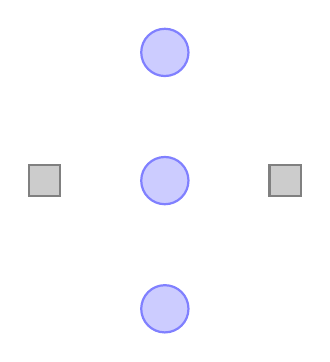
\begin{tikzpicture}
    [place/.style={circle,draw=blue!50,fill=blue!20,thick,
      inner sep=0pt,minimum size=6mm},
    transition/.style={rectangle,draw=black!50,fill=black!20,thick,
      inner sep=0pt,minimum size=4mm}]



    \node[place]      (waiting)                            {};

    \node[place]      (critical)       [below=of waiting]  {};

    \node[place]      (semaphore)      [below=of critical] {};

    \node[transition] (leave critical) [right=of critical] {};

    \node[transition] (enter critical) [left=of critical]  {};

  \end{tikzpicture}

  \caption{3~Tutorial: A~Petri-Net for Hagen,~11.}


\end{figure}
% ##################





% ##################
\begin{figure}

  \centering


  \begin{tikzpicture}


  \end{tikzpicture}

  \caption{!!! Zacząć od 3.9. 3~Tutorial: A~Petri-Net for Hagen,~12.}


\end{figure}
% ##################





% ##################
\begin{figure}

  \centering


  \begin{tikzpicture}


  \end{tikzpicture}

  \caption{3~Tutorial: A~Petri-Net for Hagen,~10.}


\end{figure}
% ##################
































% ############################
% End of the document

\end{document}
